\documentclass[11pt]{report}
\usepackage{graphicx}
\usepackage{hyperref}
\begin{document}
\begin{titlepage}
    \thispagestyle{empty}
    \title{%
    Toxic Processor \\
    \large A simplistic 4-bit processor ready to synthesis \\ 
    Version 2.0.0}
    \author{Entropy Xu \\ 
            \href{mailto:entropy.xcy@protonmail.com}{entropy.xcy@protonmail.com} }
    \maketitle
    \end{titlepage}
    \tableofcontents


    \chapter{Introduction}
    \section{Intention}
    \section{Advantages}
    \section{Limitations}
    \section{History of Revisions}


    \chapter{Design of the Processor}
    \label{chapter:design}
    \section{Overview}
    This processor is a \textbf{4-bit} \textbf{Stack machine} (0-address machine).
    \begin{itemize}
        \item The addressing width is configurable to be a multiple of 4.
        \item The stack depth is configurable to be greater than 16.
        \item The width of each Instruction is 4 bits. Thus, 16 Instructions in total.
        \item The width of each block inside the stack is 4 bits.
        \item Von Neumann Architecture: seperate data memory and code memory.
        \item Code memory and data memory are using the same addressing space.
    \end{itemize}

    \section{Data Structure}
    The name \textbf{stack machine} or equivalently 0-address machine means that 
    there is no addressable register in this machine neither do operands in the instructions. \par
    
    In order to store temporary data in this processor, we use a hardware stack to replace 
    the register file which is usually implemented by other popular processors. \par

    The 4-bit block-data-width will not limit the scalability of this processor in that addressing
    width of this processor is 4-bits but a configurable width of a multiple of 4 
    (usually 8 bits or 12 bits or 16 bits).

    \subsection{Stack for Storing Temporary Data}
    We have a stack for storing temporary data. 
    Stack is a LIFO (Last In First Out) data structure.
    Each block of the stack is a 4-bits register.
    The stack supports common operations like push and pop. For each Instruction we execute,
    we will have to read value from TOS (Top of Stack) and NTOS (Next Top of Stack), 
    and push the result of the operations to the stack.
    (Refer to Figure \ref{figure:stack_model} for the model of the stack)
    \begin{figure}[h!]
        \centering
        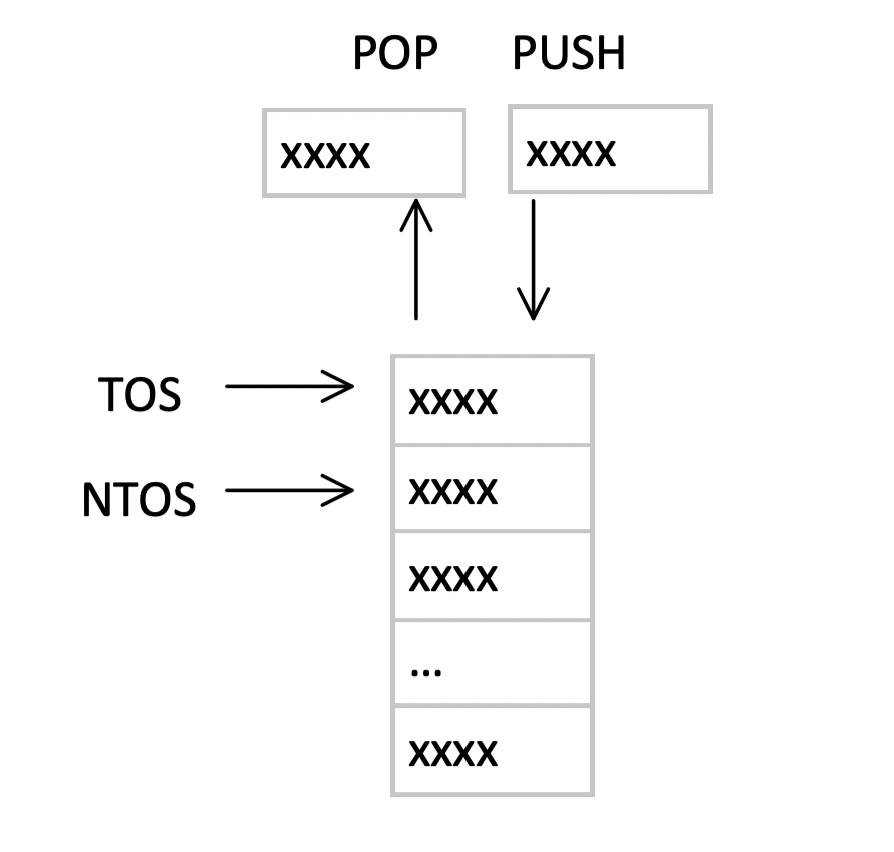
\includegraphics[scale=0.6]{Toxic_Stack_Model.png}
        \caption{Toxic Stack Model}
        \label{figure:stack_model}
    \end{figure}

    \subsection{Queue for Addressing Bus}
    We have discussed that the addressing width for the Toxic processor is configurable and 
    usually more than 4 bits. Thus, we establish a Queue as the data structure for storing
    the address of the Bus. For the length of the queue, we have $Length(Queue) = BitWidth(BusAddress) / 4 * 2$ \par
    Queue is a FIFO data structure. However, the Queue data structure we used in the Toxic 
    processor is similar to the common Queue but with some tweaks. Same as the stack, each 
    block in the Queue is a 4-bits register. The Queue should supports common operations like 
    \textbf{enqueue} and \textbf{dequeue}. Refer to Figure \ref{figure:queue_model} for the model
    of the queue and the connection with the BusAddress. Noted that, when we \textbf{enqueue}, all
    the blocks shift left one position relative to the BusAddress; when we \textbf{dequeue}, all
    the blocks shift right one position relative to the BusAddress.
    \begin{figure}[h!]
        \centering
        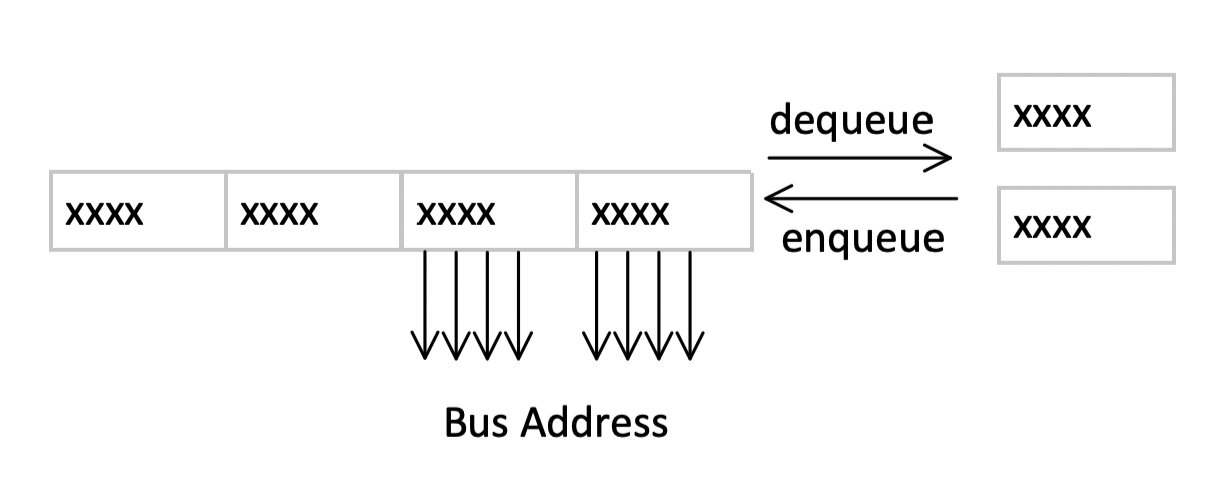
\includegraphics[scale=0.5]{Toxic_Queue_Model.png}
        \caption{Toxic Queue Model}
        \label{figure:queue_model}
    \end{figure}
    \subsection{Memory}
    The memory of the Toxic processor is accessed through Bus and only takes part of the addressing space. 
    The model of the Memory is different from common RAMs since for common RAMs, the block bit width is 1 bype (8 bits)
    while for the Toxic processor, the width of a block is half-byte (4 bits). \par
    For the Toxic processor, we assign the width of each block of the memory to be 4 bits.
    This memory model can be easily implemented using a standard memory block and would be discussed in detail in 
    Chapter \ref{chapter:implementation}.
    Detailed addressing space definitions can be found in detail in section \ref{section:addressingspace}.

    \section{Addressing Modes}
    There are three addressing modes in the Toxic processor:
    \begin{itemize}
        \item TOS (Top of Stack)
        \item NTOS (Next Top of Stack)
        \item Bus for memory and peripherals
    \end{itemize}

    \section{Addressing Space}
    These definitions for the addressing space is for the standard version of the Toxic processor.
    More versions of definitions of implementations can be found in Chapter \ref{chapter:implementation}
    \label{section:addressingspace}
    \subsection{Reserved: 0x0-0xf}
    \subsection{Code Memory: 0x10-0x7fff}
    \subsection{Data Memory: 0x8000-0xefff}
    \subsection{Peripherals: 0xf000-0xffff}

    \chapter{Instruction Set Architecture}
    \section{Instructions Map}
    \begin{table}[h]
        \begin{tabular}{|l|l|l|l|l|}
        \hline
        1:0\textbackslash{}3:2 & 00  & 01  & 11   & 10 \\ \hline
        00                     & P0  & POP & ADD  & SV \\ \hline
        01                     & P1  & DIS & NAND & LD \\ \hline
        11                     & CMP & SWP & LS   & B1 \\ \hline
        10                     & PC  & RVS & RS   & B0 \\ \hline
        \end{tabular}
    \end{table}
    For the explanation of instructions below, refer to Chapter \ref{chapter:design} for details
    about terminologies like Stack, Queue, pop, push, enqueue, dequeue, TOS, NTOS.
    \section{Push Instructions}
    \subsection{P0}
    \begin{itemize}
        \item Functionality: \textbf{Push} 0000 to stack.
        \item Expression:
        \begin{verbatim}
            Stack.push(0000);
        \end{verbatim}
    \end{itemize}

    \subsection{P1}
    \begin{itemize}
        \item Functionality: \textbf{Push} 0001 to stack.
        \item Expression:
        \begin{verbatim}
            Stack.push(0001);
        \end{verbatim}
    \end{itemize}

    \section{Stack and Bus Operation Instructions}
    \subsection{POP}
    \begin{itemize}
        \item Functionality: \textbf{Pop} from stack and
                \textbf{enqueue} the value \textbf{poped} from stack to the queue.
        \item Expression:
        \begin{verbatim}
            val = Stack.pop();
            Queue.enqueue(val);
        \end{verbatim}
    \end{itemize}

    \subsection{DIS}
    \begin{itemize}
        \item Functionality: \textbf{Pop} from the stack and discard the value.
        \item Expression:
        \begin{verbatim}
            Stack.pop();
        \end{verbatim}
    \end{itemize}

    \subsection{SWP}
    \begin{itemize}
        \item Functionality: Swap the value of \textbf{TOS} and \textbf{NTOS}.
        \item Expression:
        \begin{verbatim}
            val = Stack.ntos;
            Stack.ntos = Stack.tos;
            Stack.tos = val;
        \end{verbatim}
    \end{itemize}

    \subsection{RVS}
    \begin{itemize}
        \item Functionality: \textbf{dequeue} from the Queue and \textbf{push} the value 
                    \textbf{dequeued} to the Stack.
        \item Expression:
        \begin{verbatim}
            val = Queue.dequeue();
            Stack.push(val);
        \end{verbatim}
    \end{itemize}

    \section{Numeric Computing Instructions}
    \subsection{ADD}
    \begin{itemize}
        \item Functionality: \textbf{Push} the value of \textbf{TOS} + \textbf{NTOS}.
        \item Expression:
        \begin{verbatim}
            val = Stack.tos + Stack.ntos;
            Stack.push(val);
        \end{verbatim}
    \end{itemize}

    \subsection{NAND}
    \begin{itemize}
        \item Functionality: \textbf{Push} the value of \textbf{TOS} NAND (bit-wise) \textbf{NTOS}.
        \item Expression:
        \begin{verbatim}
            val = ~(Stack.tos & Stack.ntos);
            Stack.push(val);
        \end{verbatim}
    \end{itemize}

    \subsection{LS}
    \begin{itemize}
        \item Functionality: \textbf{Left Shift} one bit the value of \textbf{TOS}.
        \item Expression:
        \begin{verbatim}
            Stack.tos = Stack.tos << 1;
        \end{verbatim}
    \end{itemize}

    \subsection{RS}
    \begin{itemize}
        \item Functionality: \textbf{Right Shift} one bit the value of \textbf{TOS}.
        \item Expression:
        \begin{verbatim}
            Stack.tos = Stack.tos >> 1;
        \end{verbatim}
    \end{itemize}

    \section{Memory Operations Instructions}
    \subsection{SV}
    \begin{itemize}
        \item Functionality: \textbf{Save} the value of \textbf{TOS} to memory location 
                pointed by the \textbf{Bus} address.
        \item Expression:
        \begin{verbatim}
            Memory[BusAddress] = Stack.tos;
        \end{verbatim}
    \end{itemize}

    \subsection{LD}
    \begin{itemize}
        \item Functionality: \textbf{Push} the value of at memory location 
                pointed by the \textbf{Bus} address to the \textbf{Stack}.
        \item Expression:
        \begin{verbatim}
            Stack.push(Memory[BusAddress]);
        \end{verbatim}
    \end{itemize}

    \section{Branch Instructions}
    \subsection{B1}
    \begin{itemize}
        \item Functionality: Branch to the address pointed by the \textbf{Bus} 
                address if the least significant bit of \textbf{TOS} is 1.
        \item Expression:
        \begin{verbatim}
            if(Stack.tos[0] == 1)
            {
                PC = BusAddress;
            }
        \end{verbatim}
    \end{itemize}

    \subsection{B0}
    \begin{itemize}
        \item Functionality: Branch to the address pointed by the \textbf{Bus} 
                address if the least significant bit of \textbf{TOS} is 0.
        \item Expression:
        \begin{verbatim}
            if(Stack.tos[0] == 0)
            {
                PC = BusAddress;
            }
        \end{verbatim}
    \end{itemize}

    \section{Special Instructions}
    \subsection{CMP}
    \begin{itemize}
        \item Functionality: Compare \textbf{TOS} and \textbf{NTOS} with the assumption 
                that they are both signed values, push an output (described below) to the Stack.
        \item Output[0] equals 1 for \textbf{TOS} == \textbf{NTOS}, equals 0 otherwise.
        \item Output[1] equals 1 for \textbf{TOS} > \textbf{NTOS}, equals 0 otherwise.
        \item Output[2] equals 1 for \textbf{TOS} < \textbf{NTOS}, equals 0 otherwise.
        \item Output[3] equals 1 for Numeric operation having an carry, equals 0 otherwise.
        \item Expression:
        \begin{verbatim}
            output0 = Stack.tos == Stack.ntos;
            output1 = Stack.tos > Stack.ntos;
            output2 = Stack.tos < Stack.ntos;
            output3 = carry;
            Output = output0 + output1 << 1 
                    + output2 << 2 + output3 << 3;
            Stack.push(Output);
        \end{verbatim}
    \end{itemize}

    \subsection{PC}
    \begin{itemize}
        \item Important Note: This Instruction is optional for the most simplistic design.
        \item Functionality: Replace the whole \textbf{Queue} with current \textbf{PC}.
        \item Expression:
        \begin{verbatim}
            Queue = PC;
        \end{verbatim}
    \end{itemize}


    \chapter{Implementation}
    \label{chapter:implementation}
    \section{Modules List}
    \section{Data Path}


\end{document}
